%% ============================================================
%%  SFT + GRPO on Qwen3-0.6B — Project Presentation
%%  Compile with: pdflatex slides.tex  (twice for references)
%% ============================================================
\documentclass[aspectratio=169,10pt]{beamer}

% ── Theme ────────────────────────────────────────────────────
\usetheme{Madrid}
\usecolortheme{seahorse}
\setbeamertemplate{navigation symbols}{}
\setbeamertemplate{footline}[frame number]
\setbeamerfont{frametitle}{size=\large,series=\bfseries}

% ── Packages ─────────────────────────────────────────────────
\usepackage{booktabs}
\usepackage{graphicx}
\usepackage{tikz}
\usetikzlibrary{arrows.meta,shapes.geometric,positioning,fit,backgrounds}
\usepackage{xcolor}
\usepackage{amsmath}

% ── Image base path ──────────────────────────────────────────
\graphicspath{{"results/plots (3)/"}}

% ── Colours ──────────────────────────────────────────────────
\definecolor{baseblue}{RGB}{70,130,180}
\definecolor{sftoran}{RGB}{255,140,0}
\definecolor{grpogre}{RGB}{60,179,113}
\definecolor{lightgray}{RGB}{245,245,245}
\definecolor{darkgray}{RGB}{80,80,80}

% ── Helper: coloured badge ───────────────────────────────────
\newcommand{\badge}[2]{%
  \tikz[baseline=-0.6ex]\node[fill=#1,rounded corners=3pt,
    inner xsep=4pt,inner ysep=2pt,text=white,font=\footnotesize\bfseries]{#2};}

% ── Title info ───────────────────────────────────────────────
\title[SFT + GRPO on Qwen3-0.6B]{%
  Supervised Fine-Tuning and GRPO\\
  on Qwen3-0.6B for Mathematical Reasoning}
\subtitle{GSM8K · SVAMP · MMLU Evaluation}
\author{Yue Wu, Hanfu Zhao}
\date{\today}

\begin{document}

% ════════════════════════════════════════════════════════════
\begin{frame}
  \titlepage
\end{frame}

% ════════════════════════════════════════════════════════════
\begin{frame}{Outline}
  \tableofcontents
\end{frame}

% ════════════════════════════════════════════════════════════


\section{Motivation \& Objective}
\begin{frame}{Motivation \& Objective}

  \begin{columns}[T]
    \begin{column}{0.55\textwidth}
      \textbf{Question:} Can a tiny 0.6B model become a reliable
      math problem solver through fine-tuning alone?

      \vspace{0.8em}
      \textbf{Why it matters}
      \begin{itemize}
        \item Small models are cheap to run and deploy
        \item Math reasoning is a hard, structured task — a
              good benchmark for fine-tuning quality
        \item GRPO is a lightweight RL alternative to RLHF
              — no value network needed
      \end{itemize}

      \vspace{0.8em}
      \textbf{This project}
      \begin{itemize}
        \item Train \textbf{Qwen3-0.6B-Base} with SFT then GRPO
        \item Evaluate on GSM8K, SVAMP, and MMLU
        \item Use LoRA / PEFT to keep VRAM under 15 GB
      \end{itemize}
    \end{column}

    \begin{column}{0.42\textwidth}
      \begin{block}{At a Glance}
        \small
        \begin{tabular}{ll}
          \toprule
          Model        & Qwen3-0.6B-Base \\
          Fine-tuning  & LoRA (r=8, $\alpha$=16) \\
          SFT steps    & 300 \\
          GRPO steps   & 200 \\
          Train data   & GSM8K (7\,473 ex.) \\
          Eval data    & GSM8K / SVAMP / MMLU \\
          Hardware     & 2$\times$ NVIDIA T4 (15 GB) \\
          Framework    & HuggingFace + TRL \\
          \bottomrule
        \end{tabular}
      \end{block}
    \end{column}
  \end{columns}
\end{frame}

\section{Literature Review}
\begin{frame}{Literature Review: Math Reasoning in LLMs}

Recent work suggests that strong mathematical reasoning in large language models (LLMs) arises from combining
\textbf{math-specific supervision} with \textbf{reinforcement learning (RL)}. 
However, different studies assign different roles to each stage.

\begin{itemize}
    \item \textbf{DeepSeekMath (Shao et al., 2024)}
    \begin{itemize}
        \item Builds a 7B open math model using math-focused continued pretraining, instruction tuning, and GRPO-based RL.
        \item Shows that relatively small models can achieve strong reasoning performance with specialized training.
        \item Demonstrates strong results on benchmarks such as \textbf{MATH (51.7\%)} and \textbf{GSM8K}.
    \end{itemize}

    \item \textbf{Two-Stage Recipe (Yoshihara et al., 2025)}
    \begin{itemize}
        \item Proposes a sequential training strategy: \textbf{extended SFT} followed by \textbf{GRPO}.
        \item Studies the distinct contributions of supervised learning and reinforcement learning.
    \end{itemize}
\end{itemize}

Both works highlight the importance of combining supervised learning with RL, but differ in how much each stage contributes to reasoning ability.
\end{frame}
\begin{frame}{Literature Review: Role of SFT vs RL}

The two papers offer different interpretations of how reasoning ability emerges.

\begin{itemize}

\item \textbf{DeepSeekMath Perspective}
\begin{itemize}
    \item RL is a key ingredient for improving reasoning in open models.
    \item GRPO enables efficient training with verifiable rewards from math problems.
    \item However, improvements come from multiple factors:
    \begin{itemize}
        \item math-domain pretraining corpus
        \item instruction tuning
        \item RL optimization
    \end{itemize}
    making attribution difficult.
\end{itemize}

\item \textbf{Two-Stage Recipe Perspective}
\begin{itemize}
    \item \textbf{Extended SFT} (up to 10 epochs) is the main driver of accuracy.
    \item \textbf{GRPO} mainly reduces reasoning length and improves token efficiency.
    \item RL acts more as a \textbf{behavior optimizer} than a capability creator.
\end{itemize}

\end{itemize}

\textbf{Takeaway:} Domain data and SFT build reasoning capability, while RL helps refine reasoning trajectories and efficiency.
\end{frame}
% ════════════════════════════════════════════════════════════
\section{Fine-tuning Method}
\begin{frame}{SFT and GRPO}

  \begin{columns}[T]
    \begin{column}{0.48\textwidth}
      \begin{block}{\badge{sftoran}{SFT} \ Supervised Fine-Tuning}
        \begin{itemize}
          \item Cross-entropy training on
                (prompt, chain-of-thought) pairs
          \item Labels masked on prompt tokens — only the
                response contributes to the loss
          \item Teaches the model \emph{what format} to use
                and \emph{how to reason step-by-step}
          \item Fast and stable; used as the starting point for GRPO
        \end{itemize}
      \end{block}
    \end{column}

    \begin{column}{0.48\textwidth}
      \begin{block}{\badge{grpogre}{GRPO} \ Group Relative Policy Optimisation}
        \begin{itemize}
          \item Samples $G=8$ completions per prompt
          \item Computes group-normalised advantages:
                $\hat{A}_i = \frac{r_i - \bar{r}}{\sigma_r}$
          \item Maximises a clipped surrogate objective
                + KL penalty against the SFT reference model
          \item \textbf{No value network} — much cheaper than PPO
          \item Reward: correctness (1.0) + format bonus (0.5)
        \end{itemize}
      \end{block}
    \end{column}
  \end{columns}

  \vspace{0.8em}
  \begin{center}
    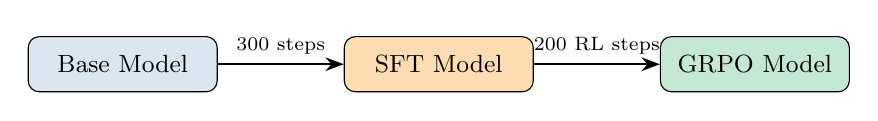
\begin{tikzpicture}[node distance=1.2cm,every node/.style={font=\small}]
      \node[draw,rounded corners,fill=baseblue!20,minimum width=2.4cm,minimum height=0.7cm] (base) {Base Model};
      \node[draw,rounded corners,fill=sftoran!30,minimum width=2.4cm,minimum height=0.7cm,right=1.6cm of base] (sft) {SFT Model};
      \node[draw,rounded corners,fill=grpogre!30,minimum width=2.4cm,minimum height=0.7cm,right=1.6cm of sft] (grpo) {GRPO Model};
      \draw[-{Stealth},thick] (base) -- node[above,font=\scriptsize]{300 steps} (sft);
      \draw[-{Stealth},thick] (sft)  -- node[above,font=\scriptsize]{200 RL steps} (grpo);
    \end{tikzpicture}
  \end{center}
\end{frame}

% ════════════════════════════════════════════════════════════
\section{Pipeline}

% ── Pipeline Slide 1: Training ───────────────────────────────
\begin{frame}{Pipeline (1/3) — Training}
  \begin{center}
  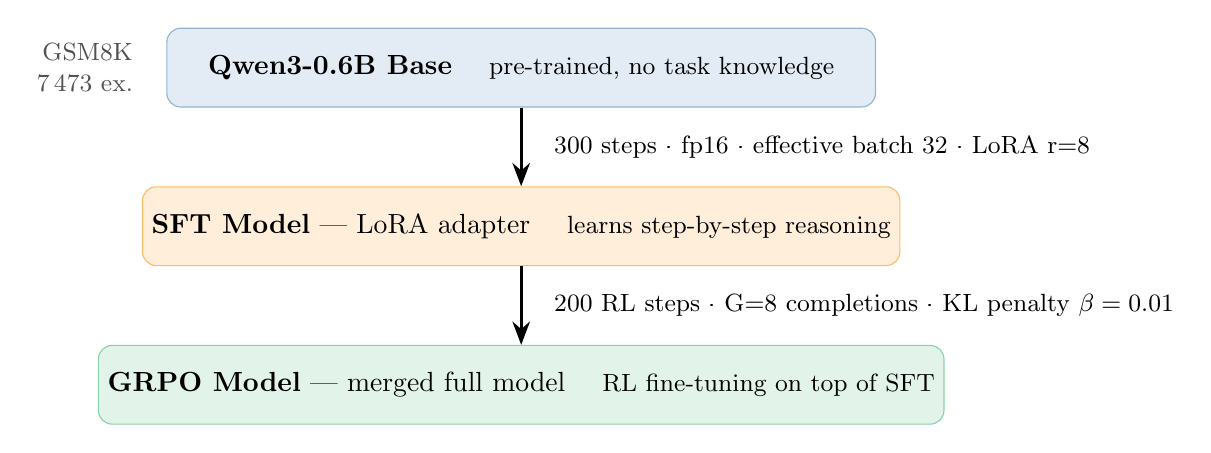
\begin{tikzpicture}[
      arr/.style={-{Stealth},thick,line width=1.2pt},
      bbase/.style={draw,rounded corners=5pt,minimum width=9cm,minimum height=1cm,
                    align=center,font=\normalsize,fill=baseblue!15,draw=baseblue!60},
      bsft/.style ={draw,rounded corners=5pt,minimum width=9cm,minimum height=1cm,
                    align=center,font=\normalsize,fill=sftoran!15,draw=sftoran!60},
      bgrpo/.style={draw,rounded corners=5pt,minimum width=9cm,minimum height=1cm,
                    align=center,font=\normalsize,fill=grpogre!15,draw=grpogre!60}
    ]
    \node[bbase] (base) {\textbf{Qwen3-0.6B Base} \quad{\small pre-trained, no task knowledge}};
    \node[bsft,below=1.0cm of base]  (sft)
          {\textbf{SFT Model} --- LoRA adapter \quad{\small learns step-by-step reasoning}};
    \node[bgrpo,below=1.0cm of sft]  (grpo)
          {\textbf{GRPO Model} --- merged full model \quad{\small RL fine-tuning on top of SFT}};

    \draw[arr] (base) -- node[right=8pt,font=\small]
          {300 steps · fp16 · effective batch 32 · LoRA r=8} (sft);
    \draw[arr] (sft)  -- node[right=8pt,font=\small]
          {200 RL steps · G=8 completions · KL penalty $\beta=0.01$} (grpo);

    \node[left=0.3cm of base,align=right,font=\small,text=darkgray]{GSM8K\\7\,473 ex.};
  \end{tikzpicture}
  \end{center}
\end{frame}

% ── Pipeline Slide 2: Evaluation ─────────────────────────────
% ── Pipeline Slide 2: Evaluation ─────────────────────────────
\begin{frame}{Pipeline (2/3) — Evaluation}

  All \textbf{3 models} are evaluated on all \textbf{3 datasets} — 9 runs in total.
  The evaluation script and prompts are identical across models;
  only the loaded weights differ.

  \vspace{0.8em}
  \begin{columns}[T]
    \begin{column}{0.48\textwidth}
      \textbf{How each model is loaded}
      \begin{itemize}
        \item \textbf{Base} — load \texttt{Qwen3-0.6B-Base} directly
        \item \textbf{SFT} — load base, then apply the LoRA adapter
              and merge the weights before inference
        \item \textbf{GRPO} — load the merged full model directly
              (base + SFT + GRPO all baked in; no adapter needed)
      \end{itemize}

      \vspace{0.6em}
      \textbf{Metrics recorded per example}
      \begin{itemize}
        \item \textbf{Correct} — predicted answer matches gold
        \item \textbf{Format} — output contains \texttt{\#\#\#\# N}
        \item \textbf{Reward} — correctness + format bonus
      \end{itemize}
    \end{column}

    \begin{column}{0.48\textwidth}
      \textbf{How answers are evaluated}

      \medskip
      \textit{GSM8K \& SVAMP (open-ended):}
      \begin{itemize}\small
        \item Generate up to 256 tokens (greedy)
        \item Extract number: look for \texttt{\#\#\#\# N} first,
              then ``Final answer: N'', then last number in text
        \item Normalize both sides (strip commas, drop \texttt{.0})
              and compare
      \end{itemize}

      \medskip
      \textit{MMLU (multiple choice):}
      \begin{itemize}\small
        \item Generate only 16 tokens
        \item Extract first A/B/C/D letter from output
        \item Compare to the correct option letter
      \end{itemize}
    \end{column}
  \end{columns}
\end{frame}
% ── Pipeline Slide 3: Analysis ───────────────────────────────
% ── Pipeline Slide 3: Analysis ───────────────────────────────
\begin{frame}{Pipeline (3/3) — Analysis \& Outputs}

  After all evaluations are complete, \texttt{analyze.py} reads the
  results from all nine JSONL files and the training logs, then
  automatically generates plots and a summary table.

  \vspace{1em}
  \begin{columns}[T]
    \begin{column}{0.48\textwidth}
      \textbf{Training diagnostics}
      \begin{itemize}
        \item SFT cross-entropy loss curve over 300 steps
        \item GRPO mean reward, KL divergence, and policy-gradient
              loss over 200 RL steps
      \end{itemize}
    \end{column}
    \begin{column}{0.48\textwidth}
      \textbf{Evaluation results}
      \begin{itemize}
        \item Accuracy and format rate for all three models on GSM8K
        \item Side-by-side GSM8K vs SVAMP accuracy comparison
        \item MMLU accuracy per subject to check for forgetting
        \item Answer length and reward distributions
      \end{itemize}
    \end{column}
  \end{columns}

  \vspace{1em}
  \begin{block}{}
    \small
    All outputs are saved to \texttt{images/} and zipped for download.
    No manual post-processing is needed --- the full analysis runs in
    under two minutes after training completes.
  \end{block}

\end{frame}
% ════════════════════════════════════════════════════════════
\section{Datasets}
\begin{frame}{Datasets}

  \begin{columns}[T]
    \begin{column}{0.32\textwidth}
      \begin{block}{\badge{sftoran}{GSM8K}}
        \begin{itemize}\small
          \item 8.5K grade-school word problems
          \item Train: 7\,473 · Test: 1\,319 (eval: 500)
          \item Chain-of-thought ending with \texttt{\#\#\#\# N}
          \item \textbf{Purpose}: in-distribution training \& eval
        \end{itemize}
      \end{block}
    \end{column}

    \begin{column}{0.32\textwidth}
      \begin{block}{\badge{grpogre}{SVAMP}}
        \begin{itemize}\small
          \item 1\,000 adversarial math problems
          \item Same difficulty as GSM8K but different phrasing
          \item Eval: 500 examples
          \item \textbf{Purpose}: out-of-distribution generalisation
        \end{itemize}
      \end{block}
    \end{column}

    \begin{column}{0.32\textwidth}
      \begin{block}{\badge{baseblue}{MMLU (subset)}}
        \begin{itemize}\small
          \item 3 subjects, 150 each:
            \begin{itemize}\scriptsize
              \item High School Mathematics
              \item Elementary Mathematics
              \item World History
            \end{itemize}
          \item \textbf{Purpose}: catastrophic forgetting check
        \end{itemize}
      \end{block}
    \end{column}
  \end{columns}

  \vspace{0.7em}
  \begin{center}
    \small\textit{Chain-of-thought prompt example (GSM8K):}
    \medskip

    \colorbox{lightgray}{\parbox{0.82\textwidth}{%
      \texttt{Question: Janet has 16 eggs. She eats 3 for breakfast. How many does she sell?}\\
      \texttt{Answer: Let's think step by step.}\\
      \texttt{She has 16 - 3 = 13 eggs left.}\\
      \texttt{{\color{grpogre}\#\#\#\# 13}}
    }}
  \end{center}
\end{frame}

% ════════════════════════════════════════════════════════════
\section{Results}
\begin{frame}{GSM8K Results — In-Distribution Math}

  \begin{columns}[T]
    \begin{column}{0.48\textwidth}
      \includegraphics[width=\linewidth]{accuracy_comparison.png}
    \end{column}

    \begin{column}{0.48\textwidth}
      \includegraphics[width=\linewidth]{format_rate_comparison.png}
    \end{column}
  \end{columns}

  \vspace{0.4em}
  \begin{center}
    \small
    \begin{tabular}{lccc}
      \toprule
      & Base & SFT & GRPO \\
      \midrule
      Accuracy   & 37.2\% & \textbf{51.6\%} & 49.2\% \\
      Format rate & 0.0\% & 95.4\% & \textbf{96.0\%} \\
      Avg reward  & 0.37  & 0.99   & 0.97   \\
      \bottomrule
    \end{tabular}
    \quad
    \begin{minipage}{0.42\textwidth}\small
      SFT gives the biggest accuracy jump (+14 pp).\\
      GRPO reinforces structured output format.
    \end{minipage}
  \end{center}
\end{frame}

% ════════════════════════════════════════════════════════════
\begin{frame}{SVAMP Results — Generalisation}

  \begin{columns}[T]
    \begin{column}{0.48\textwidth}
      \includegraphics[width=\linewidth]{svamp_accuracy.png}
    \end{column}

    \begin{column}{0.48\textwidth}
      \includegraphics[width=\linewidth]{gsm8k_vs_svamp.png}
    \end{column}
  \end{columns}

  \vspace{0.4em}
  \begin{center}\small
    \begin{tabular}{lccc}
      \toprule
      & Base & SFT & GRPO \\
      \midrule
      Accuracy & 71.4\% & 62.2\% & 61.8\% \\
      Format   & 0.0\%  & 99.6\% & 99.8\% \\
      \bottomrule
    \end{tabular}
    \quad
    \begin{minipage}{0.42\textwidth}\small
      Base already solves SVAMP well.\\
      Fine-tuning causes mild over-specialisation ($-9$ pp)\\
      but SFT and GRPO are nearly identical.
    \end{minipage}
  \end{center}
\end{frame}

% ════════════════════════════════════════════════════════════
\begin{frame}{MMLU Results — Catastrophic Forgetting Check}

  \begin{columns}[T]
    \begin{column}{0.56\textwidth}
      \includegraphics[width=\linewidth]{mmlu_forgetting.png}
    \end{column}

    \begin{column}{0.41\textwidth}
      \begin{block}{Key Takeaways}
        \begin{itemize}
          \item All models score $\sim$9\% — below random chance (25\%)
          \item \textbf{Not forgetting} — the base model is also $\sim$9\%
          \item 0.6B parameters is too small for 4-choice academic MCQ
          \item \textbf{No measurable degradation} from fine-tuning
        \end{itemize}
      \end{block}

      \vspace{0.5em}
      \begin{center}
        \small
        \begin{tabular}{lcc}
          \toprule
          Model & Overall & $\Delta$ vs Base \\
          \midrule
          Base  & 8.7\%  & — \\
          SFT   & 8.7\%  & 0.0 pp \\
          GRPO  & 9.0\%  & +0.3 pp \\
          \bottomrule
        \end{tabular}
      \end{center}
    \end{column}
  \end{columns}
\end{frame}

% ════════════════════════════════════════════════════════════
\begin{frame}{SFT Training Curve}

  \begin{columns}[T]
    \begin{column}{0.62\textwidth}
      \includegraphics[width=\linewidth]{sft_training_curve.png}
    \end{column}

    \begin{column}{0.35\textwidth}
      \begin{block}{SFT Details}
        \begin{itemize}
          \item 300 optimiser steps
          \item Batch size 2, grad accum 16\\
                (effective batch = 32)
          \item fp16 mixed precision
          \item Gradient checkpointing
          \item Loss decreases steadily,\\
                confirming stable training
        \end{itemize}
      \end{block}
    \end{column}
  \end{columns}
\end{frame}

% ════════════════════════════════════════════════════════════
\begin{frame}{GRPO Training Curves}

  \begin{columns}[T]
    \begin{column}{0.62\textwidth}
      \includegraphics[width=\linewidth]{grpo_training_curves.png}
    \end{column}

    \begin{column}{0.35\textwidth}
      \begin{block}{Reward Design}
        \small
        \begin{tabular}{lc}
          \toprule
          Condition & Reward \\
          \midrule
          Correct + \texttt{\#\#\#\#} & 1.5 \\
          Correct only   & 1.0 \\
          \texttt{\#\#\#\#} only  & 0.5 \\
          Neither        & 0.0 \\
          \bottomrule
        \end{tabular}
      \end{block}

      \vspace{0.5em}
      \begin{itemize}\small
        \item Mean reward rises \textbf{0.86 → 1.06}
        \item High variance is normal in GRPO —
              group sampling is noisy
        \item KL divergence stays small —
              model stays close to SFT reference
      \end{itemize}
    \end{column}
  \end{columns}
\end{frame}

% ════════════════════════════════════════════════════════════
\begin{frame}{Answer Length Distribution}

  \begin{center}
    \includegraphics[width=0.82\linewidth]{answer_length_distribution.png}
  \end{center}

  \vspace{0.2em}
  \begin{center}\small
    Correct answers tend to be longer — more reasoning steps lead to the right answer.
  \end{center}
\end{frame}

\begin{frame}{Reward Distribution}

  \begin{center}
    \includegraphics[width=0.65\linewidth]{reward_distribution.png}
  \end{center}

  \vspace{0.2em}
  \begin{center}\small
    SFT and GRPO shift the reward distribution clearly rightward compared to the base model.
  \end{center}
\end{frame}

% ════════════════════════════════════════════════════════════
% ──────────────────────────────────────────────────────────
%   ADDITIONAL EXPERIMENTS  (Hanfu's contribution)
% ──────────────────────────────────────────────────────────
% ════════════════════════════════════════════════════════════

\section{Additional Experiments}

\begin{frame}{Additional Experiments — Overview}
  Three further experiments to address key design decisions
  required by the project brief.

  \vspace{1em}
  \begin{enumerate}
    \item \textbf{Prompt Design Comparison}\\
          Does the prompt format matter? Compare three strategies.
    \item \textbf{DoRA vs LoRA}\\
          Does Weight-Decomposed LoRA outperform standard LoRA?
    \item \textbf{Step-by-Step Reasoning Validity}\\
          Are the intermediate arithmetic steps actually correct?
  \end{enumerate}

  \vspace{1em}
  \begin{center}\small
    \textit{All experiments use the same Qwen3-0.6B model, GSM8K dataset,
    and hyperparameters for fair comparison.}
  \end{center}
\end{frame}

% ── Prompt Design ─────────────────────────────────────────
\begin{frame}{Experiment 1 — Prompt Design Comparison}

  \begin{columns}[T]
    \begin{column}{0.48\textwidth}
      \begin{block}{Three Strategies}
        \begin{itemize}
          \item \badge{baseblue}{direct} Bare question, no guidance
          \item \badge{sftoran}{cot} ``Let's think step by step''
                (Chain-of-Thought)
          \item \badge{grpogre}{rules} Explicit math rules
                (+, $-$, $\times$, $\div$) then step-by-step
        \end{itemize}
      \end{block}

      \vspace{0.6em}
      \textbf{Why it matters}
      \begin{itemize}\small
        \item Prompt design is listed as a key decision
        \item Same model weights — only the prompt changes
        \item Tests whether explicit instructions help a small model
      \end{itemize}
    \end{column}

    \begin{column}{0.48\textwidth}
      \begin{block}{Prompt Examples}
        \footnotesize
        \textbf{direct:}\\
        \texttt{Question: Janet has 16 eggs...\\Answer:}

        \vspace{0.4em}
        \textbf{cot:}\\
        \texttt{You are a helpful assistant...\\
        Question: Janet has 16 eggs...\\
        Answer: Let's think step by step.}

        \vspace{0.4em}
        \textbf{rules:}\\
        \texttt{You are a math tutor. Rules:\\
        - Addition (+): combining...\\
        - Subtraction (-): difference...\\
        Question: Janet has 16 eggs...\\
        Answer: Let's solve step by step.}
      \end{block}

      \vspace{0.3em}
      \includegraphics[width=\linewidth]{prompt_comparison.png}
    \end{column}
  \end{columns}
\end{frame}

% ── DoRA vs LoRA ──────────────────────────────────────────
\begin{frame}{Experiment 2 — DoRA vs LoRA}

  \begin{columns}[T]
    \begin{column}{0.52\textwidth}
      \begin{block}{What is DoRA?}
        \begin{itemize}\small
          \item LoRA: $W' = W + BA$ \quad ($B \in \mathbb{R}^{d \times r}$, $A \in \mathbb{R}^{r \times k}$)
          \item DoRA decomposes weight into \textbf{magnitude} and \textbf{direction}:
                $W' = m \cdot \frac{W + BA}{\|W + BA\|}$
          \item Extra learnable magnitude scalar $m$ per layer
          \item Inspired by Weight Normalization (Salimans \& Kingma, 2016)
        \end{itemize}
      \end{block}

      \vspace{0.5em}
      \begin{block}{Experimental Setup}
        \small
        \begin{tabular}{ll}
          \toprule
          & LoRA \quad / \quad DoRA \\
          \midrule
          Rank $r$     & 8 \\
          Alpha $\alpha$ & 16 \\
          Target modules & all attn + MLP \\
          Steps        & 300 \\
          Batch size   & 2 $\times$ 16 = 32 \\
          Precision    & fp16 \\
          \bottomrule
        \end{tabular}

        \vspace{0.3em}
        \textit{Identical hyperparameters — only \texttt{use\_dora} differs.}
      \end{block}
    \end{column}

    \begin{column}{0.45\textwidth}
      \begin{block}{GSM8K Results}
        \begin{center}
        \begin{tabular}{lcc}
          \toprule
          Method & Accuracy & Format \\
          \midrule
          LoRA (SFT)  & \textbf{51.6\%} & 95.4\% \\
          DoRA (SFT)  & \textit{TBD}    & \textit{TBD} \\
          \bottomrule
        \end{tabular}
        \end{center}
        \small\textit{(Fill in after running on Kaggle)}
      \end{block}

      \vspace{0.5em}
      \begin{block}{Key Question}
        Does the magnitude--direction decomposition in DoRA
        help a 0.6B model learn math reasoning better than
        standard LoRA?
      \end{block}
    \end{column}
  \end{columns}
\end{frame}

% ── Reasoning Validity ────────────────────────────────────
\begin{frame}{Experiment 3 — Step-by-Step Reasoning Validity}

  \begin{columns}[T]
    \begin{column}{0.48\textwidth}
      \textbf{Motivation}\\
      Final-answer accuracy only tells us \emph{what} the model got right,
      not \emph{how}. A model could reach the right answer through
      wrong intermediate steps (lucky cancellation).

      \vspace{0.6em}
      \textbf{Method}
      \begin{itemize}\small
        \item Extract every arithmetic expression from the completion\\
              e.g.\ \texttt{16 - 3 = 13}, \texttt{5 * 4 = 20}
        \item Verify each calculation independently
        \item Classify completions into four quadrants:
      \end{itemize}

      \vspace{0.4em}
      \footnotesize
      \begin{tabular}{l|cc}
        & Correct answer & Wrong answer \\
        \hline
        Valid reasoning  & \textcolor{grpogre}{\textbf{Best}} & Unlucky \\
        Invalid reasoning & Lucky   & \textcolor{red}{\textbf{Worst}} \\
      \end{tabular}
    \end{column}

    \begin{column}{0.48\textwidth}
      \begin{block}{Metrics}
        \begin{itemize}\small
          \item \textbf{Step accuracy}: fraction of arithmetic steps
                that are mathematically correct
          \item \textbf{Reasoning validity rate}: fraction of completions
                where \emph{all} extracted steps are correct
          \item \textbf{Avg steps}: reasoning depth per completion
        \end{itemize}
      \end{block}

      \vspace{0.4em}
      \includegraphics[width=\linewidth]{reasoning_validity.png}

      \vspace{0.3em}
      \begin{center}\small
        \textit{Compares Base vs SFT vs GRPO reasoning quality}
      \end{center}
    \end{column}
  \end{columns}
\end{frame}

% ════════════════════════════════════════════════════════════
\section{Summary}
\begin{frame}{Summary \& Discussion}

  \begin{columns}[T]
    \begin{column}{0.48\textwidth}
      \begin{block}{What We Achieved}
        \begin{itemize}
          \item Fine-tuned Qwen3-0.6B on 2×T4 GPUs
          \item \textbf{SFT}: +14 pp on GSM8K, 95\% format adoption
          \item \textbf{GRPO}: reward rises +24\%, format improves further
          \item \textbf{No catastrophic forgetting} on MMLU
          \item \textbf{Prompt comparison}: CoT vs direct vs rules
          \item \textbf{DoRA vs LoRA}: same setup, method comparison
          \item \textbf{Reasoning validity}: verified arithmetic steps
        \end{itemize}
      \end{block}
    \end{column}

    \begin{column}{0.48\textwidth}
      \begin{block}{Limitations \& Future Work}
        \begin{itemize}
          \item GRPO slightly below SFT ($-$2.4 pp): more RL steps needed
          \item SVAMP drop: format over-specialisation on GSM8K style
          \item MMLU: 0.6B too small; 3B+ needed for meaningful scores
          \item \textbf{Next steps}:
            \begin{itemize}\small
              \item More GRPO steps (500+)
              \item Mix SVAMP into training data
              \item Try Qwen3-1.7B or 3B
            \end{itemize}
        \end{itemize}
      \end{block}
    \end{column}
  \end{columns}

  \vspace{0.5em}
  
\end{frame}

\begin{frame}{Summary}
    \begin{center}
    \begin{tabular}{lcccc}
      \toprule
      & \multicolumn{2}{c}{GSM8K} & SVAMP & MMLU \\
      \cmidrule(lr){2-3}
      Model & Acc. & Format & Acc. & Acc. \\
      \midrule
      Base  & 37.2\% & 0.0\%  & 71.4\% & 8.7\% \\
      SFT   & \textbf{51.6\%} & 95.4\% & \textbf{62.2\% }& 8.7\% \\
      GRPO  & 49.2\% & \textbf{96.0\%} & 61.8\% & \textbf{9.0\%} \\
      \bottomrule
    \end{tabular}
  \end{center}
\end{frame}
% ════════════════════════════════════════════════════════════
\begin{frame}[plain]
  \begin{center}
    \vspace{2em}
    {\Huge \textbf{Thank You}}\\[1em]
    {\large Questions?}\\[2em]
    \small
    \begin{tabular}{ll}
      Model   & Qwen3-0.6B-Base (Alibaba Cloud) \\
      Dataset & GSM8K, SVAMP, MMLU \\
      Code    & github.com/202520030411/Fine-tuning-and-GRPO-on-Qwen \\
      Tools   & HuggingFace Transformers, PEFT, TRL, PyTorch \\
    \end{tabular}
  \end{center}
\end{frame}

\end{document}
